%%%%%%% Damit fangen wir nächste Woche an %%%%%%%%
\newpage
\newpage
\section[Einführung in die Gebietsintegrale]{Mehrdimensionale Integrale}
\subsection{Theoretisches Baukasten}
Um uns mit mehrdimensionalen Integralen zu beschäftigen, müssen wir zuerst gewisse theoretische Begriffe einführen.
\begin{Def}{Charakteristische Funktion}
Sei $A\subseteq \R^n$. Die charakteristische Funktion \textit{oder auch} \red{Indikatorfunktion} der Teilmenge $A$ ist die Funktion
$$1_A:\R^n \rightarrow \R \mbox{ mit } x\rightarrow \begin{cases}1, x\in A \\
0, x\notin A\end{cases}$$
\end{Def}
\begin{Def}{Quader}
Ein \red{Quader} $Q\subseteq \R^n$ ist das Produkt $I_1\times \cdots \times I_n$ von $n$ beschränkten, nicht-leeren Intervallen $I_\mu \subseteq \R$.
\end{Def}
\begin{Beispiel}{Quader in $\R^1$}
Quader in $\R^1$ sind also die Intervale $(a,b)$, $[a,b]$, $(a,b]$ und $[a,b)$. \\
\end{Beispiel}
\begin{Def}{Volumen eines Quaders}
Das (n-dimensionale) Volumen eines solchen Quaders ist die nicht-negative reelle Zahl
$$v(Q)=v_n(Q)=\prod_{\mu = 1}^n |I_\mu|=\prod_{\mu = 1}^n (b_\mu - a_\mu)$$
\end{Def}
\begin{Def}{Treppenfunktion}
Eine Funktion $\varphi:\R^n \rightarrow \C$ heißt \red{Treppenfunktion auf $\R^n$}, wenn es endlich viele paarweise \textbf{disjunkte} Quader gibt, sodass
\begin{enumerate}[a)]
    \item die Funktion $\varphi$ auf jedem Quader $Q_k$ konstant ist,
    \item $\varphi(x)=0$ für alle $x$ außerhalb von Quadern.
    \end{enumerate}
Außerdem lassen sich Treppenfunktionen als endliche Linearkombination charakteristischer Funktionen von disjunkten Quadern schreiben
$$\varphi=\sum_{k}c_k 1_{Q_k} \mbox{ mit $c_k\in \C$ und $Q_k$ ist ein Quader}$$ 
\end{Def}
Wir kommen nun zu den sehr wichtigen Begriff der Hüllreihen.
\begin{Def}{Hüllreihe}
Gegeben sei $f:\R^n\rightarrow\C\cup \{\infty\}$. Eine \red{Hüllreihe} zu $f$ ist eine Reihe
$$\Phi=\sum_{k=1}^\infty c_k1_{Q_k} \mbox{ mit $c_k\in \R$}$$
wobei $Q_k$ \textbf{offene} Quader im $\R^n$ sind und für jedes $x\in\R^n$ gilt
$$|f(x)|\leq \Phi(x) = \sum_{k=1}^\infty c_k1_{Q_k}(x)$$
Der \red{Inhalt} der Hüllreihe ist definiert als
$$I(\Phi) = \sum_{k=1}^\infty c_k v(Q_k)$$
\end{Def}

\begin{Beispiel}{Folge von Hüllreihen}
Seien $a, k\in \R$ und $f:\R\rightarrow\R$ definiert als $f(x)=\begin{cases}0, x\neq a && k, x=a\end{cases}$. Wir sollen zu dieser Funktion eine Folge von Hüllreihen, $\Phi_n$, konstruieren, die gegen Null konvergiert. \\
Wir wissen, dass $\Phi = \sum_{k=1}^\infty c_k 1_{Q_k}$, aber auch, dass $c_k=0$ für jeden Quader außer für den einen, in dem sich $a$ befindet (da ist $c_k=k$).
\red{Achtung!} Dieses Beispiel ist noch unvollständig!
\end{Beispiel}
\begin{Def}{$L^1$-Halbnorm}
Unter der \red{$L^1$-Halbnorm} von $f:\R^n\rightarrow\C\cup \{\infty\}$ versteht man das Infimum
$$||f||_1=\inf\{I(\Phi) |\mbox{ $\Phi$ Hüllreihe zu $f$} \}=\int |f|dx$$
\end{Def}
\begin{Satz}{Satz}{Eigenschaften einer Halbnorm}
Für die Funktionen $f_1, f_2: \R^n\rightarrow \C\cup\{\infty\}$ und ein $c\in\C$ gilt
\begin{enumerate}
\item $||c\cdot f||_1 = |c|\cdot ||f||_1$
\item $|f_1| \leq |f_2|  \implies ||f_1||_1 \leq ||f_2||_2$
\item $||\sum_{k=1}^\infty |f_k| ||_1\leq \sum_{k=1}^\infty ||f_k||_1$
\end{enumerate}
\end{Satz}
\subsection{Lebesgue-Integral}
Mit den obigen theoretischen Werkzeug können wir nun endlich das Lebesgue-Integral definieren.
\begin{Def}{Lebesgue-Integral}
Eine Funktion $f:\R^n\rightarrow\C\cup\{\infty\}$ heißt \red{Lebesgue-integrierbar} über $\R^n$, wenn es eine Folge von Treppenfunktionen $\varphi_k$ gibt mit
$$\lim_{k\rightarrow \infty}||f-\varphi_k||_1=0$$
In diesem Fall schreiben wir das \red{Lebesgue-Integral}
$$\int fdx = \int f(x) d^nx = \int_{\R^n} f(x)dx = \lim_{k\rightarrow\infty} \varphi_k(x)dx\in\C$$
\end{Def}
\begin{Satz}{Satz}{Bedingte Gleichheit der Riemann und Lebesgue Integrale}
Sei $A=[a,b]$ ein kompaktes Intervall und $f$ eine über $A$ Riemann-integrierbare Funktion. Dann ist $f$ über $A$ Lebesgue-integrierbar und das Lebesgue-Integral und das Riemann-Integral sind gleich.
\end{Satz}
Der folgende zwei Sätze sind sehr wichtig in der Theorie der Gebietsintegrale. Im Skript stehen der kleiner und großer Satz von Fubini, wir schreiben hier aber die allgemeine Version aus T. Arens, also guckt euch auch das Skript nochmal an.
\begin{Satz}{Satz}{Kleiner Satz von Beppo Levi}
Sei $f:\R^n\rightarrow \R\cup \{\infty\}$ und sei $(\varphi_k)$ eine monoton wachsende oder fallende Folge von Treppenfunktionen, so dass
\begin{enumerate}[a)]
    \item $(\varphi_k)$ punktweise gegen $f$ konvergiert
    \item die Folge ($\int \varphi_k dx$) der Integrale der Treppenfunktionen beschränkt ist.
    Dann ist $f$ integrierbar und es gilt
    $$\int f dx=\lim_{k\rightarrow \infty}\int \varphi_k dx$$
\end{enumerate}
\end{Satz}
\begin{Satz}{Satz}{Satz von Fubini}
Sind $I\subseteq R^p$ und $J\subseteq R^q$ (möglicherweise unbeschränkte) Quader sowie $f\in L(Q)$ eine auf dem Quader $Q=I\times J \subseteq R^{p+q}$ integrierbare (oder mindestens stetig beschränkte) Funktion, so gibt es Funktionen $g\in L(I)$ und $h\in L(J)$ mit
$$g(x)=\int_J f(x,y) dy \mbox{ für fast alle $x\in I$}$$
$$h(y)=\int_I f(x,y)dx \mbox{ für fast alle $y\in J$}$$
Ferner ist 
$$\int_R f(x,y) d(x,y) = \int_I\int_J f(x,y) dy dx = \int_I g(x) dx$$
$$=\int_J\int_I f(x,y) dx dy = \int_J h(y) dy$$

\end{Satz}
\begin{Beispiel}{Anwendung vom Satz von Fubini}
Wir wollen auch für eine kompliziertere Funktion, aber noch stets definiert auf einem Rechteck, die interierten Integrale berechnen. Dazu betrachten wir $R=(0,\frac{\pi}{2})\times (0,\frac{\pi}{2}$ und die Funktion $f:R\rightarrow \R$, die durch
$$f(x)=\sin(x_1+2x_2), \mbox{ $x=(x_1,x_2)\in R$}$$
gegeben ist.
\begin{center}
    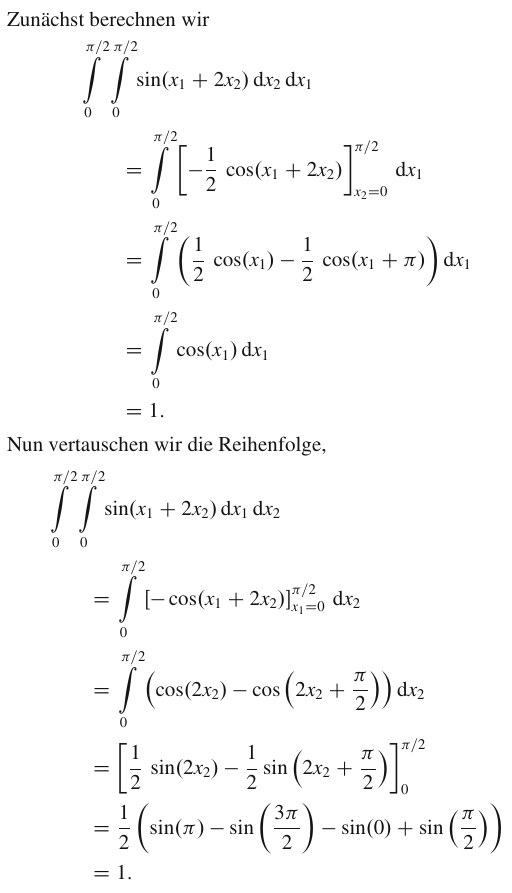
\includegraphics[width=.6\textwidth]{Dateien/Fubini1.png}
\end{center}
\end{Beispiel}
\begin{Beispiel}{Fubini ist nicht immer anwendbar}
\begin{center}
    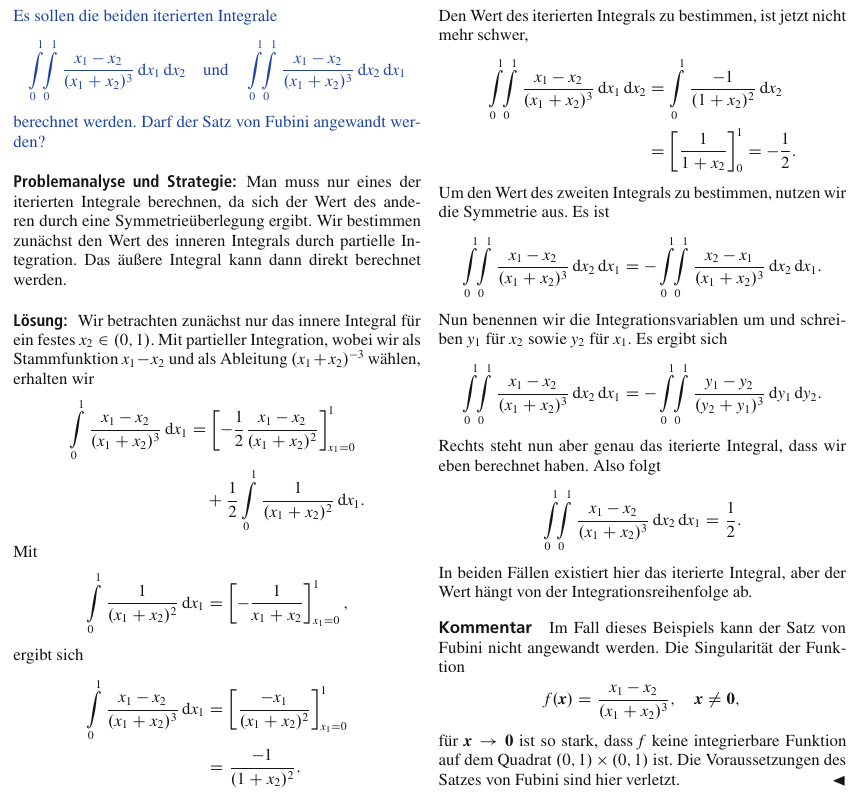
\includegraphics[width=\textwidth]{Dateien/Fubini2.png}
\end{center}
\end{Beispiel}